\documentclass[letterpaper,oneside,12pt,spanish]{book}

\usepackage[utf8]{inputenc}
\usepackage[spanish]{babel}
\usepackage[T1]{fontenc}
\usepackage{tocbibind} % Bibliografía en el indice
\usepackage{titlesec} % Posibilidad de editar los formatos de chapter
\usepackage{amsmath,amssymb,mathrsfs} % Matemáticas varias
\usepackage{hyperref} %Esto te hace un pequeño esquemita al lado
\usepackage{listings}
\usepackage{anysize} 
\usepackage{algorithmic} % Para pseudocódigo de algoritmos
\usepackage{algorithm}
\usepackage{appendix} % Para tener apéndice en vez de capítulos
\usepackage{verbatim}



% --- Arreglos varios para la inclusion de imagenes
\usepackage[pdftex]{graphicx}
\usepackage{subfigure}
\usepackage{graphicx}
\usepackage[usenames,dvipsnames]{color}
\DeclareGraphicsExtensions{.png,.jpg,.pdf,.mps,.gif,.bmp}

% --- Para las dimensiones de los márgenes etc
% \frenchspacing \addtolength{\hoffset}{-1.5cm}
% \addtolength{\textwidth}{3cm} \addtolength{\voffset}{-2.5cm}
% \addtolength{\textheight}{4cm}
\marginsize{3.8cm}{2.5cm}{2cm}{2cm} 

\setlength{\parskip}{0.7em}

% --- Para el encabezado
\usepackage{fancyhdr}
\fancyhead[R]{UTFSM}\fancyhead[L]{} \fancyfoot[C]{\thepage}
\pagestyle{fancy}

% --- Para las tablas
\renewcommand{\tablename}{Tabla}
\renewcommand{\listtablename}{Índice de tablas}

% --- Para los apendices
\renewcommand{\appendixname}{Anexos}
%\renewcommand{\appendixtocname}{Anexos}
%\renewcommand{\appendixpagename}{Anexos}
% -------------------------------------------------------- %

\title{Estado del Arte: Web browsers bajo ataques y sus mecanismos de Seguridad.}
\author{Paulina Andrea Silva Ghio}

\lstset{ %
language=C,                % choose the language of the code
basicstyle=\footnotesize,       % the size of the fonts that are used for the code
numbers=left,                   % where to put the line-numbers
numberstyle=\footnotesize,      % the size of the fonts that are used for the line-numbers
stepnumber=0,                   % the step between two line-numbers. If it's 1 each line 
                                % will be numbered
numbersep=5pt,                  % how far the line-numbers are from the code
backgroundcolor=\color{white},  % choose the background color. You must add \usepackage{color}
showspaces=false,               % show spaces adding particular underscores
showstringspaces=false,         % underline spaces within strings
showtabs=false,                 % show tabs within strings adding particular underscores
frame=single,	                % adds a frame around the code
tabsize=2,	                % sets default tabsize to 2 spaces
captionpos=b,                   % sets the caption-position to bottom
breaklines=true,                % sets automatic line breaking
breakatwhitespace=false,        % sets if automatic breaks should only happen at whitespace
title=\lstname,                 % show the filename of files included with \lstinputlisting;
                                % also try caption instead of title
escapeinside={\%*}{*)},         % if you want to add a comment within your code
morekeywords={*,...}            % if you want to add more keywords to the set
}

\begin{document}
\frontmatter
\begin{titlepage}

\begin{center}

\textsc{\Large Universidad Técnica Federico Santa María}\\
\textsc{\large Departamento de Informática}\\
\textsc{\large Valparaíso, Chile}\\[1.5cm]

% Upper part of the page

\includegraphics[width=0.3\textwidth]{figures/utfsm.jpg}\\[1cm]    

% Title
{ \huge ???? }\\[2cm]

% Author and supervisor
\text{\Large Paulina Andrea Silva Ghio}\\[2cm]
\text{\large Memoria para obtar al título de: Ingeniera Civil Informática}\\[3cm]
\text{\large Profesor Guía: Raúl Monges}\\
\text{\large Profesor Correferente: Javier Cañas}

\vfill

% Bottom of the page
{\large \today}

\end{center}

\end{titlepage}
 

\begin{flushright}  
\null \vspace{\stretch{1}}
\emph{} 
\end{flushright}
\newpage 
\chapter{Agradecimientos}
\label{chap:agrad}

\section*{Agradecimientos}

 
\newpage 
% Resumen a grandes rasgos de lo existente (resumen del estado del arte y resumen del trabajo realizado)

\chapter{Resumen}
\label{chap:resumen}

El uso del Internet en la vida cotidiana ya es parte de la mayoría del mundo. Para cada necesidad de información el usuario puede buscar en Internet aquello que lo aqueja, desde comprar tickets para una película, realizar reuniones por videoconferencia y muchas otras tareas que en el pasado no eran necesarias, pero que hoy en día su uso es imperante; como las redes sociales. La Web 2.0 ha sido gran colaboradora de éste éxito en la vida de las personas, entregando las herramientas para que los contenidos que los usuarios necesiten estén disponibles de diversas formas y en tiempo real.

Junto con éste desarrollo en la forma de interactuar con la Internet, parte de la responsabilidad de que existan la tienen los desarrolladores que crean Software de acuerdo a los requerimientos de sus clientes. Dentro de las necesidades de los clientes, algunos equipos de Desarrollo de Software tienen casi siempre en cuenta ciertos requerimientos no funcionales que permiten conservar ciertos atributos en el Sistema a crear, como: Confidencialidad, Integridad, No Repudio y Disponibilidad. Sin embargo, muchas veces por los costos y poco tiempo que poseen, los atributos mencionados no son salvaguardados. En consecuencia el producto final, podría llegar a tener serias consecuencias tanto en el Cliente como en los Usuarios que podrían llegar a usar el Sistema.

El Objetivo de esta Memoria es concretar un Estado del Arte que analice el funcionamiento y estructura (componentes) del Web Browser, e investigar los peligros en que se puede encontrar un usuario al usar la aplicación \textit{killer}\footnote{Web Browsers}. Además se desea construir una Arquitectura de Referencia que permita comprender los componentes que interactúan en el browser y desarrollar patrones de mal uso de estos artefactos; mencionando los componentes utilizados para que los ataques se lleven a cabo. Finalmente se desea clasificar los riesgos y mecanismos de defensa (mitigación) de los navegadores Web, para poder obtener un panorama general de cómo los Web Browser protegen al usuario.


\section*{Abstract}


 
\markboth{}{}
\newpage
\tableofcontents 
\newpage
\renewcommand{\sectionmark}[1]{\markright{\thesection\ #1}}

\mainmatter
\label{chap:intro}


\section{Motivación}
\label{chap:intro.1}


\section{Contribuciones}
\label{chap:intro.2}

\section{Estructura del Documento}
\label{chap:intro.3}


\newpage
\chapter{Estado del Arte: El Web Browser}
\label{chap:chap2}


\section{Organizaciones}
\label{chap:Orgs}

\subsection{OWASP}
Desde el 2066 la Open Web Application Security Project ha estado entregando pautas de còmo desarrollar aplicaciones web, en un ambiente que constantemente está cambiando. Su objetivo principal es buscar y combatir las causas de inseguridad en el desarrollo de Software, proporcionando una gran cantidad de documentación y herramientas aquellos que lo necesiten y no sean expertos en seguridad. Para lograr su cometido, todos los años la OWASP entrega una lista de los Riesgos y Threats más críticos sobre la seguridad de las Aplicaciones Web, de manera de preveer que Desarrolladores de Sistemas o programadores generen vulnerabilidades en el Software que crean.


\subsection{IEEE CSD}

%\subsection{}


\section{Same Origin Policy}
\label{chap:SOP}

Este importante concepto nace a partir del Modelo de Seguridad detrás de una Aplicación Web, al mismo tiempo que es el mecanismo más básico que el Browser tiene para protegerse de las amenazas que aparecen en el día a día, haciendo un poco más complicado el trabajo de realizar un \textit{exploit}. \textbf{Same Origin Policy} o \textbf{SOP} define lo que es un \textbf{Origen}, compuesto por el \textit{esquema}, el \textit{host/dominio} y \textit{puerto} de la URL. Esta política permite que un Web Browser aisle los distintos recursos obtenidos por las páginas web y que solo permita la ejecución de \textit{Script} que pertenezcan a un misno \textbf{Origen}. 

\textbf{SOP} puede distinguir entre la información que envía y recibe el Web Browser, y solo se aplicará la política a los elementos externos que se soliciten dentro de una página web (recepción de la información). Esta imposibilidad de recibir información de un \textbf{Origen} diferente al del recurso actual, permite disminuir la superficie de ataque y la posibilidad de explotar alguna vulnerabilidad en el sistema donde reside el Browser. Sin embargo, \textbf{SOP} no pone ninguna restricción sobre la información que el usuario puede enviar hacia otros. 


%Ver libro de Browser hacker handbook

\section{HTML: HyperText Markup Language}
\label{chap:HTML}
HTML \cite{htmlSpec} es conocido por ser un \textit{Simple Markup Language} o lenguage de marcado simple, usado principalmente para crear documentos de hypertextos que son posibles de portar desde una plataforma a otra, sin problemas de compatibilidad. Un documento HTML sigue el estandar dado por SGML o \textit{Standard Generalized Markup Language}, que entrega una semántica apropiada para representar una gran variedad de información y aplicaciones. Un documento HTML consiste de un árbol de elementos y texto, cada uno de esos elementos es denotado por un tag inicial y uno final; estos tags pueden ir aninados y la idea es no se superponen entre ellos. Un HTML User Agent o Browser consume el HTML y lo parsea para crear un árbol DOM, que es la representación en memoria del documento HTML.
Para poder crear una Aplicación interactiva y segura con HTML, es necesario evadir la creación de vulnerabilidades por donde los atacantes podrían comprometer la integridad del sitio o del usuario que descarga el recurso HTML del sitio atacado. Típicos errores que deben ser evitados cuando se usa scripting con HTML, es que los scripts en HTML tienen una semántica run to completion, esto quiere decir que el browser ejecutará el script mucho antes de que se realice el parsing del documento o gatillar un evento; este tipo de comportamiento es el que los atacantes aprovechan para realizar sus ataques.

\section{Webworkers}

\section{}

\section{HTTP}
\label{chap:HTTP}

\subsection{Comunicación en HTTP}
\label{chap:comunHTTP}

\subsubsection{postMessage}
\label{chap:postmessage}

\subsubsection{XMLHttpRequest}
\label{XMLHR}

\subsubsection{WebSockets}
\label{WebSockets}


\newpage
\chapter{El Web Browser} %buscar referencia
%se hablará de los componentes y tecnologías usadas por los browser conocidos
\label{chap:chap3}


\section{Google: Google Chrome y Google Chromium}
La misión de Google es organizar la información del mundo y lograr que sea útil y accesible para todo el mundo. Esta gran empresa partió como un búscador y rápidamente llegó a ser dueño de la mayor parte de búsquedas en el mundo. Tiene servicios de almacenamiento en la nube, correo electrónico, \textit{e-wallet} y otros más. Google ha sido responsable por la construcción del Navegador Web \textbf{Google Chrome} y \textit{Google Chromium}, siendo la segunda la versión open source.

La arquitectura de Chrome o Chromium se basa principalmente en dos módulos: el Browser Kernel y el Rendering Engine, cómo se puede ver en la Figura \ref{fig:archG}.

\begin{figure}[h!t]
    \begin{center}
        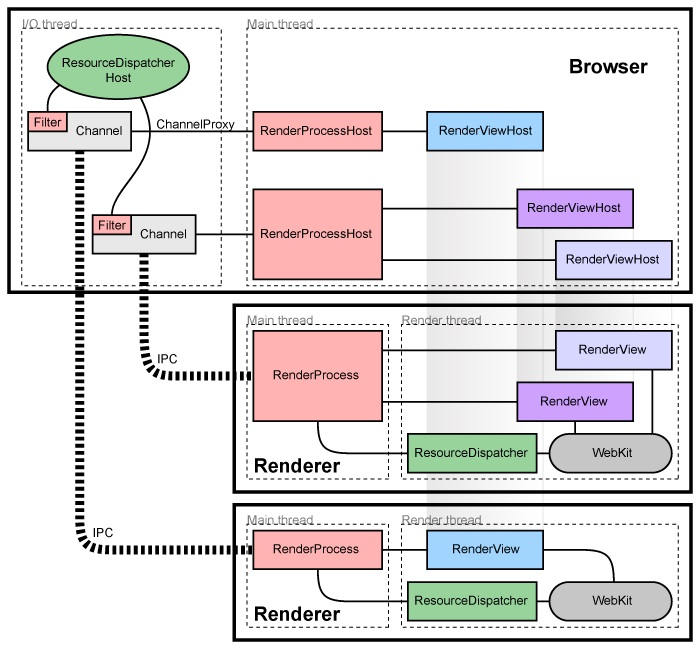
\includegraphics[scale=0.5]{figures/archGC.jpg}
      %\caption{Representación conceptual de una Nube con Eucalyptus. La especificación de las partes y su explicación se ve en \ref{sec:chap2.4.2}. Fuente \cite{EucalyptusOverview}}
      \label{fig:archG}
    \end{center}
\end{figure}

Én la documentación de Google Chromium \cite{multiProcArchG}, que es base para Google Chrome, afirma que la arquitectura soporta para cada tab un proceso nuevo, de manera de hacer al Browser más robusto y modularizar el sistema para evitar ciertas amenazas de seguridad. El proceso principal es llamado \textit{Browser Process/Kernel/Engine} y se encarga de la \textit{User Interface}, manejo de las tabs y los procesos de los \textit{plug-in}. Cada tab es asociado a un Rendering Engine, éstos tienen restricciones de acceso (\textit{Sandoboxing}) a los demas y al sistema, lo que permite que exista una protección de la memoria y un control de acceso. En \cite{barth2008security} se explica que el objetivo principal de esta arquitectura es poder mitigar ataques muy severos sin tener que sacrificar la compatibilidad con los sitios web ya existentes. Para lograr el objetivo Google ha ganado muchas lecciones de cómo realizar esto \cite{reis2009browser}, pues explican que un gran desafío en la seguridad es proteger a los usuarios de los atacantes que se aprovechan de las vulnerabilidades y debilidades de los clientes web-browsers. En su arquitectura modular se puede ver que se intenta proveer una seguridad que evita afectar la compatibilidad con otros sitios. La arquitectura comentada se basa en dos decisiones de diseño: La arquitectura depende en el Rendering Engine para aquellos componentes de alto riesgo como JavaScript, el parser de HTML y la creación de DOM para hacer cumplir SOP; al estar rodeados por un Sandboxing hace que el Rendering Engine se comporte como una caja negra. 


Google Chrome expone en \cite{reis2009browser} que existen ciertas lecciones que han ido utilizando para mejorar la calidad de su browser. Estas son:

\begin{itemize}
	\item Reducción de las vulnerabilidades de seguridad, se basa en la aislación de ciertos componentes y la reducción de privilegios de ciertas tareas en el browser. La aislación lo lograron con la creación del Rendering Engine y el Browser Kernel, que tienen como objetivo proteger la data del sistema de archivos. Si bien esto puede no entregar muchos beneficios a una aplicación web, si lo hace en el usuario del browser.
	\item Reducir la ventana de vulnerabilidades, la actualización del browser se hace cada cierto tiempo de forma automática para así cubrir las vulnerabilidades que van apareciendo.
	\item Reducción de la frecuencia de exposición, Google trabaja con StopBadware.org para entregar una mayor seguridad al descubrir nuevos tipos de ataques y vulnerabilidades relacionadas con el browser.
\end{itemize}


\subsection{Safe Browsing API and Content-Agnostic Malware Prevention}
	%Safe Browsing API es inefectiva contra ataques de Social Eng Malware, citas: rowSecSEMBlock
	%Abrams2013: 	The	NSS	analyst	brief, “Cybercrime	Kill	Chain	vs.	Defense	Effectiveness,” demonstrates	that	holes	in	one	layer	of	defense	are	often	not	 closed	by	secondary	and	tertiary technologies. Google	augments	its Safe	Browsing	API	with	additional	download	protection	that	is	seven	times	more	effective	than	the	Safe	Browsing	API.		
\subsection{Sandboxing}
En el desarrollo de \cite{barth2008security} se define un modelo de amenazas donde se enumeran las habilidades que debería de tener un atacante y los objetivos de estos, para así caracterizar y evaluar las propiedades de seguridad necesarias para evitar que los atacantes cumplan su objetivo. Una propiedad importante que hacen destacar en el estudio es cómo aislar ciertos procesos que pueden ser aprovechados por los atacantes y ofrece una forma para poder mitigar esto: Sandboxing. El Sandboxing de Google Chrome previene al atacante de leer o escribir en el sistema de archivos del usuario, dejando al Principal Web con los privilegios necesarios para parsear un HTML/XML y ejecutar código JavaScript. Sin embargo esta arquitectura no imposibilita al atacante a atacar otros sitios web si es que el Rendering Engine fue comprometido, lo que puede convertirse en una amenaza muy grande para otros sitios web.

\subsection{Actualizaciones Periódicas}

\subsection{Address Space Layout Randomization (ASLR)}

\subsection{Privacy Settings: Do Not Track and Third-Party Cookies}


\section{Microsoft}
Internet Explorer es el navegador grafico predeterminado por Microsoft y que su primera versión 1.0 fue realizada en 1995. IE es una derivación de Spyglass Mosaic desarrolado por la NCSA (National Center for Supercomputing Applications). En primera instancia fue un navegador que podría ser obtebido si era comprado como complemento de \textit{Microsoft Plus!} o mediante la versión \textit{OEM} de Windows 95. Desde la tercera versión de IE, en 1996, que esta se lanzó de forma gratuita.
        
        La arquitectura de este navegador es modular y permite al desarrollador por utilizar los recursos para crear diferentes funcionalidades, ejemplo de esto son: toolbars, Microsoft Active X controls, etc. En la Figura \ref{fig:archIE} \cite{webpag3} se puede ver los principales componentes de la architectura del browser mencionado. IE utiliza \textit{COM} o \textit{Component Object Model} una interfaz binaria standard para componentes de software introducida por Microsoft en 1993 y que permite una comunicación entre procesos/componentes de software provenientes de la familia de software de Microsoft. \textit{COM} es similar a otras tecnologías de interfaz de componentes de software ( Component Software Interface Technologies) cómo CORBA y Java Beans. El uso de \textit{COM} gobierna la forma la interacción de los componentes que se comunicann y permite que haya un reuso y extensibilidad de estos.
        
        \begin{figure}[h!t]
		    \begin{center}
				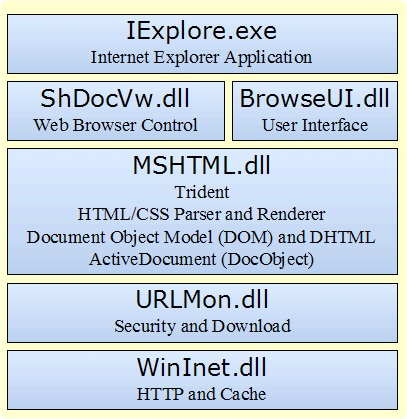
\includegraphics[scale=0.65]{figures/IEArch.jpg}
		      %\caption{Representación conceptual de una Nube con Eucalyptus. La especificación de las partes y su explicación se ve en \ref{sec:chap2.4.2}. Fuente \cite{EucalyptusOverview}}
		      \label{fig:archIE}
		    \end{center}
		\end{figure}

        
        El ejecutable IExplore.exe es la base para el corazón del navegador \textit{Mshtml.dll} que se encarga del \textit{parsing} tanto de \textit{CSS} como del \textit{HTML} así como también de la función de renderizado de la página en el navegador; tiene también la tarea de alojar otros componentes dependiendo del contenido del HTML parseado, cómo JScript, XML Data, etc. Con codename \textit{Trident}, expone su interfaz para poder ser alojado por el componente \textit{Shdocvw.dll}, llamado también WebBrowser Control, que se encarga de poder dar funcionalidad, navigabilidad y un historial al browser, permitiendo que sea alojada facilmente en una \textit{Aplicación Windows}. La interfaz de usuario es proveída por \textit{Browsui.dll}. Cuando se realiza una descarga de un recurso, \textit{Urlmon.dll} pasa por una serie de pasos para asegurar que el tipo de archivo calce con el tipo \textit{MIME} declarado por el servidor. Finalmente, \textit{WinInet.dll} se encarga de implementar los protocolos de aplicación HTTP y FTP, agregando también el manejo del cache del browser.
        
        La arquitectura de Internet Explorer, basada en la tecnología \textbf{COM}, permite extender sus capacidade, por ejemplo: \textbf{Mediante Extensiones del browser}, \textbf{Extensiones de Contenido} y \textbf{Alojo y Reuso}.

\subsection{SmartScreen}

\subsection{App Rep}

\subsection{Privacy Settings: Do Not Track and Third-Party Cookies}

\section{Mozilla}

Mozilla fue creado a partir del navegador \textit{Netscape} en 1998, el cuál ha sido rediseñado en varias ocasiones. Las metas de diseño que Mozilla desee en el navegador son:
        \begin{itemize}
            \item Renderizado rápido de las páginas web.
            \item Fuerte apoyo a los estandares web como la W3C.
            \item Interoperabilidad en las diversas plataformas.
        \end{itemize}
        
        \begin{figure}[h!t]
		    \begin{center}
				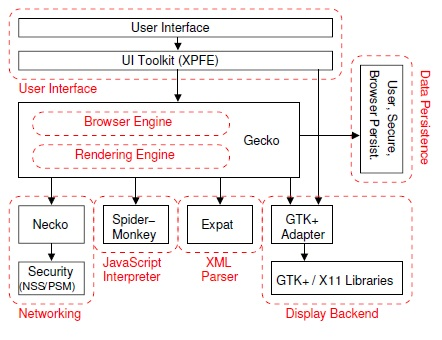
\includegraphics[scale=0.8]{figures/archMoz.jpg}
		      %\caption{Representación conceptual de una Nube con Eucalyptus. La especificación de las partes y su explicación se ve en \ref{sec:chap2.4.2}. Fuente \cite{EucalyptusOverview}}
		      \label{fig:archM}
		    \end{center}
		\end{figure}
        
        La arquitectura de este browser puede ser vista en la Figura \ref{fig:archM} donde se pueden observar los siguientes componentes:
        \begin{itemize}
            \item La interfaz de usuario, puede ser reutilizada para otras aplicaciones.
            \item La persistencia de los datos, tanto de bookmarks como de data de bajo nivel como el \textit{cache}.
            \item EL \textit{Rendering Engine}, permite el renderizado de documentos HTML/XML aún cuando estos estén mal formados. Este Engine es capaz de renderizar la interfaz de la aplicación multi-plataforma.
        \end{itemize}
        La arquitectura de Mozilla se distingue de las demás en que la visualización especificada por la plataforma y la librería de \textit{widgets} son usados directamente en el navegador, lo que minimiza el costo necesario para soportar diferentes plataformas.
        
\subsection{Componentes}
	\subsubsection{Safe Browsing}
		%ocupan la tecnología de google


\subsection{Privacy Settings: Do Not Track and Third-Party Cookies}

%tipo de arquitectura
%mecanismos de defensa

\section{Evolución y Seguridad en el Browser}
%Usar referencias varga2013evolution, EvoBrowSecNSS, browSecPhish, browSecPrivSett, rowSecSEMBlock, silic2010security, barth2008security, reis2009browser, reis2009isolating, barth2009securing, barth2010protecting, Carlini12, liu2012chrome, utakrit2009review, barth2009secure, Accuvant11, Li12, Yu07, Zalewsk08, alcorn2014browser, sansInstInfoSec, 

\newpage
\chapter{Arquitectura de Referencia del Browser}
\label{chap4:ArqRefBrowser}

%A partir de proposals y soluciones existentes se obtienen los elementos necesarios.


\section{Casos de Uso de Browser}
	\subsection{Stakeholders (actores) y Concerns de estos}

	\subsection{Casos de Uso}

		\subsubsection{Actor 1: XXX}

%			\begin{enumerate}
%				\item
%			\end{enumerate}

		\subsubsection{Actor 2: XXX}

\section{Patrón Browser}


\newpage
\chapter{Patrones de Mal Uso}
\label{chap5:MisusePatt}

\section{Identificando Amenazas}
\label{chap5:IdenThreat}


\section{Template de Patrones de Mal Uso}
\label{chap5:TemplateMP}


%\section{Escuchar Tráfico}


%\section{Robo de Datos privados por medio de extensión mal configurada}
\newpage
\chapter{Discusión}
\label{chap6:Disc}
\newpage
\chapter{Conclusiones}
\label{chap7:conclusion}


\section{Contribuciones}
\label{chap7:contrib}

\section{Trabajo Futuro}
\label{chap7:Futuro}

%\backmatter
%\addcontentsline{toc}{chapter}{References}
\bibliography{ref}
\bibliographystyle{unsrt}

\appendix
\chapter{Anexos}
\label{Anexos}

%\label{Anexo2}

\section{asdf}


\end{document}